\documentclass[11pt,a4j]{jsarticle}
\usepackage{float,array,booktabs,here}
\usepackage{amsmath}
\usepackage{bm}
\usepackage[dvipdfmx]{graphicx}
% \usepackage[whole]{bxcjkjatype}%日本語もコンパイル可にする.
%\usepackage[dvipdfmx,hiresbb]{graphicx}
\usepackage[top=25truemm,bottom=25truemm,left=25truemm,right=25truemm]{geometry}

\title{Computer Vision}
\author{81819433 開放環境科学専攻情報工学専修 修士1年 飯塚 健介}
\date{\today}
\begin{document}
    \maketitle
    \section{section name}
    \subsection{subsection name}

    \begin{figure}[H]
      \centering
      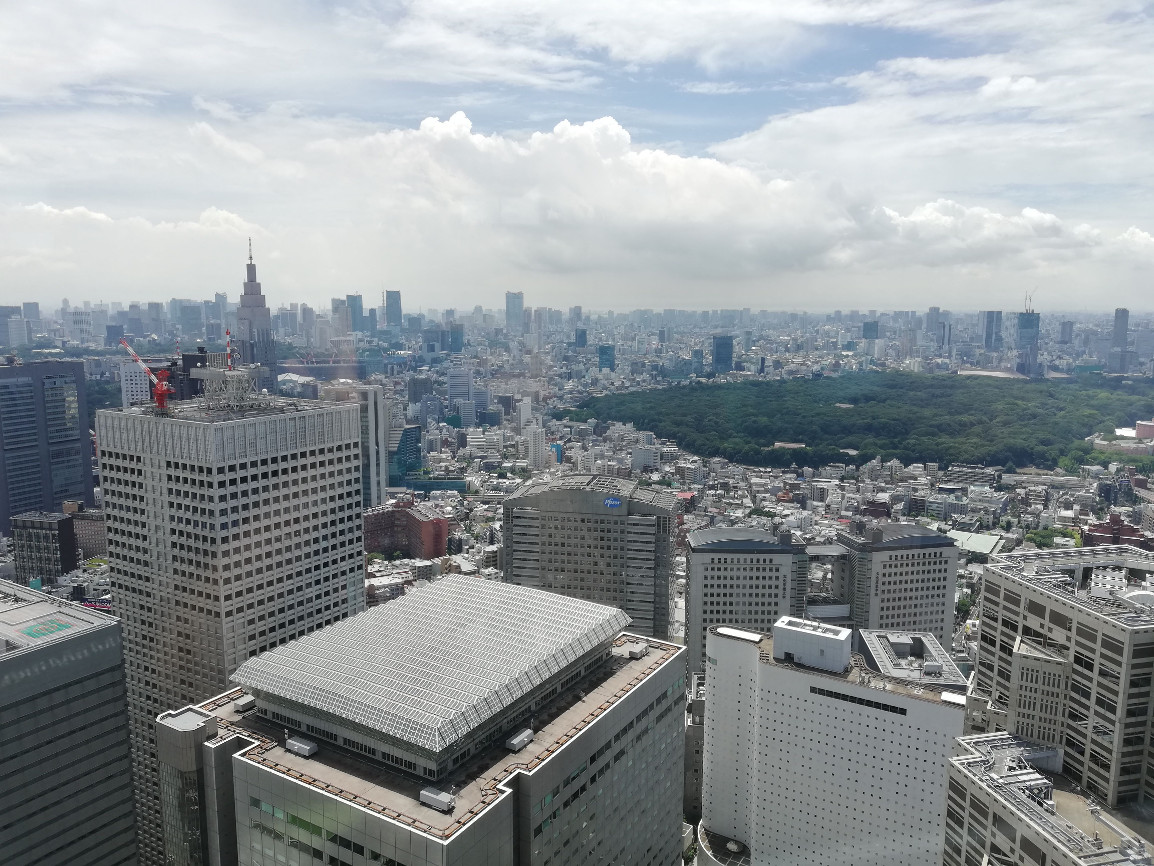
\includegraphics[clip,width=4.0cm]{img/metro.jpg}
      \caption{都庁南展望台からの写真\label{fig:cute}}
    \end{figure}

    \begin{equation}
        s\left(
        \begin{array}{c}
            u \\
            v \\
            1
        \end{array}
        \right) =
        \left(
    \begin{array}{cccc}
      P_{11} & P_{12} & P_{13} & P_{14}\\
      P_{21} & P_{22} & P_{23} & P_{24} \\
      P_{31} & P_{32} & P_{33} & P_{34} \\
    \end{array}
        \right)
        \left(
        \begin{array}{c}
            X \\
            Y \\
            Z \\
            1
        \end{array}
        \right)
        \label{eq:projection_matrix}
    \end{equation}

\end{document}
